\section{Results and discussion} \label{sec:results_and_discussion}
% some sort of visualisation of the results from research and/or results from the implementation of the mobile app
Lorem ipsum dolor sit amet.


Regarding the soHappy smile detection machine learning model, the following
result is present: After the training was finished, it was evaluated with the
test data. As Figure \ref{fig:training_result} shows, the accuracy detecting a
smile as a smile is about 98\%, with an overall evaluation accuracy of about 
94.5\%.

\begin{figure}
  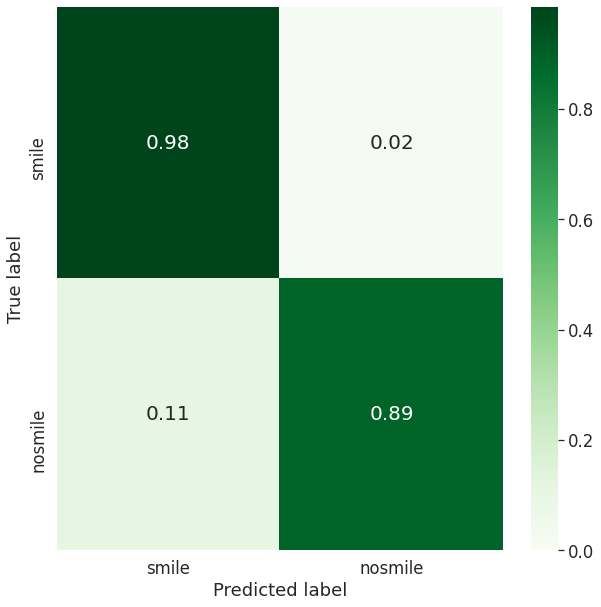
\includegraphics[width=\linewidth]{figures/training_result.png}
  \caption{Headmap }
  \label{fig:training_result}
\end{figure}

While those numbers look promising, using this model in production shows
room for improvement. Sometimes it is not enough to smile with a closed
mouth, instead an open mouth is required.

In the future, the soHappy model could be improved by improving the machine 
learning architecture. Also an bigger dataset including more photographs of
people smiling with mouth closed could significantly improve the performance.